%% This Beamer template is based on the one found here: https://github.com/sanhacheong/stanford-beamer-presentation, and edited to be used for Stanford ARM Lab

\documentclass[10pt]{beamer}
%\mode<presentation>{}

\usepackage{media9}
\usepackage{amssymb,amsmath,amsthm,enumerate}
\usepackage[utf8]{inputenc}
\usepackage{array}
\usepackage[parfill]{parskip}
\usepackage{graphicx}
\usepackage{caption}
\usepackage{subcaption}
\usepackage{bm}
\usepackage{amsfonts,amscd}
\usepackage[]{units}
\usepackage{listings}
\usepackage{multicol}
\usepackage{multirow}
\usepackage{tcolorbox}
\usepackage{physics}
%encoding
%--------------------------------------
\usepackage[T1]{fontenc}
\usepackage[utf8]{inputenc}
%--------------------------------------

%Portuguese-specific commands
%--------------------------------------
\usepackage[portuguese]{babel}
%--------------------------------------

%Hyphenation rules
%--------------------------------------
\usepackage{hyphenat}
\hyphenation{mate-mática recu-perar}
%--------------------------------------

% Enable colored hyperlinks
\hypersetup{colorlinks=true}

% The following three lines are for crossmarks & checkmarks
\usepackage{pifont}% http://ctan.org/pkg/pifont
\newcommand{\cmark}{\ding{51}}%
\newcommand{\xmark}{\ding{55}}%

% Numbered captions of tables, pictures, etc.
\setbeamertemplate{caption}[numbered]

%\usepackage[superscript,biblabel]{cite}
\usepackage{algorithm2e}
\renewcommand{\thealgocf}{}

% Bibliography settings
\usepackage[style=ieee]{biblatex}
\setbeamertemplate{bibliography item}{\insertbiblabel}
\addbibresource{references.bib}

% Glossary entries
\usepackage[acronym]{glossaries}
\newacronym{ML}{ML}{machine learning}
\newacronym{HRI}{HRI}{human-robot interactions}
\newacronym{RNN}{RNN}{Recurrent Neural Network}
\newacronym{LSTM}{LSTM}{Long Short-Term Memory}


\theoremstyle{remark}
\newtheorem*{remark}{Remark}
\theoremstyle{definition}

\newcommand{\empy}[1]{{\color{darkorange}\emph{#1}}}
\newcommand{\empr}[1]{{\color{cardinalred}\emph{#1}}}
\newcommand{\examplebox}[2]{
	\begin{tcolorbox}[colframe=darkcardinal,colback=boxgray,title=#1]
		#2
\end{tcolorbox}}

\usetheme{Stanford} 
\def \i  {\item}
\def \ai {\item[] \quad \arrowbullet}
\newcommand \si[1]{\item[] \quad \bulletcolor{#1}}
\def \wi {\item[] \quad $\ \phantom{\Rightarrow}\ $}
\def \bi {\begin{itemize}\item}
\def \ei {\end{itemize}}
\def \be {\begin{equation*}}
\def \ee {\end{equation*}}
\def \bie {$\displaystyle{}
\def \eie {{\ }$}}
\def \bsie {\small$\displaystyle{}
\def \esie {{\ }$}\normalsize\selectfont}
\def \bse {\small\begin{equation*}}
\def \ese {\end{equation*}\normalsize}
\def \bfe {\footnotesize\begin{equation*}}
\def \efe {\end{equation*}\normalsize}
\renewcommand \le[1] {\\ \medskip \lefteqn{\hspace{1cm}#1} \medskip}
\def \bex {\begin{example}}
\def \eex {\end{example}}
\def \bfig {\begin{figure}}
\def \efig {\end{figure}}
\def \btheo {\begin{theorem}}
\def \etheo {\end{theorem}}
\def \bc {\begin{columns}}
\def \ec {\end{columns}}
\def \btab {\begin{tabbing}}
\def \etab {\end{tabbing}\svneg\svneg}
\newcommand \col[1]{\column{#1\linewidth}}
\def\vneg  {\vspace{-5mm}}
\def\lvneg {\vspace{-10mm}}
\def\svneg {\vspace{-2mm}}
\def\tvneg {\vspace{-1mm}}
\def\vpos  {\vspace{5mm}}
\def\lvpos {\vspace{10mm}}
\def\svpos {\vspace{2mm}}
\def\tvpos {\vspace{1mm}}
\def\hneg  {\hspace{-5mm}}
\def\lhneg {\hspace{-10mm}}
\def\shneg {\hspace{-2mm}}
\def\thneg {\hspace{-1mm}}
\def\hpos  {\hspace{5mm}}
\def\lhpos {\hspace{10mm}}
\def\shpos {\hspace{2mm}}

\logo{
\includegraphics[height=0.4in]{./images/logoufjf10.png}}

% commands to relax beamer and subfig conflicts
% see here: https://tex.stackexchange.com/questions/426088/texlive-pretest-2018-beamer-and-subfig-collide
\makeatletter
\let\@@magyar@captionfix\relax
\makeatother

\newcommand{\code}[1]{\textcolor{red} {\textit{#1}}} %comentarios

\title[Reunião de Orientação 06]{Reunião de Orientação 06}
%\subtitle{Subtitle Of Presentation}

%\beamertemplatenavigationsymbolsempty

\begin{document}
	
	\author[Modelagem Computacional]{
		\begin{tabular}{c} 
			\Large
			Igor Pires dos Santos\\
			\footnotesize \href{mailto:igor.pires@ice.ufjf.br}{igor.pires@ice.ufjf.br}\\
			\textbf{Orientador:} Rafael Bonfim
		\end{tabular}
		\vspace{-4ex}}
	
	\institute{
		\vskip 5pt
		\begin{figure}
			\centering
			\begin{subfigure}[t]{0.5\textwidth}
				\centering
				
\includegraphics[height=0.33in]{images/logoufjf1}
			\end{subfigure}%
			~ 
			\begin{subfigure}[t]{0.5\textwidth}
				\centering
				
\includegraphics[height=0.33in]{./images/PGMC.png}
			\end{subfigure}
		\end{figure}
		\vskip 5pt
		Programa de Pós-Graduação em Modelagem Computacional\\
		Universidade Federal de Juiz de Fora\\
		\vskip 3pt
	}
	
	% \date{June 15, 2020}
	\date{\today}
	
	\begin{noheadline}
		\begin{frame}\maketitle\end{frame}
	\end{noheadline}
	
	\setbeamertemplate{itemize items}[default]
	\setbeamertemplate{itemize subitem}[circle]
	
	\begin{frame}
		\frametitle{Sumário} % Table of contents slide, comment this block out to remove it
		\tableofcontents % Throughout your presentation, if you choose to use \section{} and \subsection{} commands, these will automatically be printed on this slide as an overview of your presentation
	\end{frame}
	
	\section{Introdução}
	\begin{frame}[allowframebreaks]
		\frametitle{Introdução}
		
		\begin{itemize}
			\item A construção de modelos de árvores arteriais é importante para a realização de estudos hemodinâmicos. Neste trabalho, apresentam-se: 
			\item (i) um esquema analítico para o cálculo das características locais das ondas de fluxo e pressão em modelos de árvores arteriais 1D 
			\item (ii) um ambiente computacional desenvolvido para a simulação e visualização dos resultados no tocante à construção de modelos e estudos hemodinâmicos. Os resultados obtidos neste trabalho estão condizentes com dados numéricos relatados na literatura.
			
		\end{itemize}
		
	\end{frame}
	
	\section{Modelo Matemático}
	\begin{frame}[allowframebreaks]
		\frametitle{Modelo Matemático}
		
		\begin{itemize}
			\item \textbf{Árvore proposta}
			\item Árvore extraída do artigo Duan \& Zamir.
			
		\end{itemize}
		
		\framebreak
		
		\begin{itemize}
			\item \textbf{Duan \& Zamir}
			\item 2 Artérias terminais.
			\item 6 segmentos totais (2 pares idênticos).
			\item Considerando o caso não-viscoso e  $\phi = 0$
			\item Fase um (7 variáveis) + Fase Dois (5 variáveis)
			
		\end{itemize}
		
		\framebreak
		
		\begin{itemize}
			\item \textbf{Parâmetros de Entrada (r(cm),L(cm),$\rho$(g/$cm^3$),E(g/$cm*s^2$),f(Hz),$\epsilon$,$\mu_0$,$\phi_0$)}
			\item $ f =3.65$Hz.
			\item [0] = $(r = 0.65)$, $(L = 25)$,$(\rho = 0.96)$ e $(E = 4.8 * 10^6)$.
			\item [1] = $(r = 0.45)$, $(L = 11)$,$(\rho = 1.134)$ e $(E = 10^7)$.
			\item [2] = $(r = 0.3)$, $(L = 12)$,$(\rho = 1.172)$ e $(E = 10^7)$.
			\item [3] = $(r = 0.2)$, $(L = 10)$,$(\rho = 1.235)$ e $(E = 10^7)$.
			
		\end{itemize}
		
		\framebreak
		
		\begin{itemize}
			\item $ h = 0.1 * r $.
			\item $ C = \sqrt{\frac{Eh}{\rho 2 r}}$.
			\item $ \omega = 2 \pi f$.
			\item $ \beta = \omega \frac{L}{c}$.
			\item $ Y = \frac{\pi r^2}{\rho c}$.
			
		\end{itemize}
		
		
		\framebreak
		
		\begin{itemize}
			\item \textbf{Ângulo do fase}:
			\item $ E_c = \|E_c\|\exp{i\phi}$.
			\item $ \phi = \phi_0 (1 - \exp{-w})$.
			
		\end{itemize}
		
		
		\framebreak
		
		\begin{itemize}
			\item \textbf{Viscoso}:
			\item $ c_v = c\sqrt{\epsilon}$.
			\item $ Y_v = Y\sqrt{\epsilon}$.
			\item $ \alpha = R \sqrt{\frac{\omega \rho}{\mu}}$.
			\item $ \phi = \phi_0 (1 - \exp{-w})$.
			\item $ \epsilon = 1 - F_{10}(\alpha)$.
			\item $ F_{10}(\alpha) = \frac{2J_1(i^{\frac{3}{2}} \alpha)}{\alpha i^{\frac{3}{2}} J_0(i^{\frac{3}{2}} \alpha)}$.
			
		\end{itemize}
		
		\framebreak
		
		\begin{itemize}
			\item \textbf{Reflection Coefficient <<complex>> e Admittance <<complex>>}
			\item Se folha $ R = 0 $, senão $ R = \frac{Y - (Ye_r + Ye_l)}{Y + (Ye_r Ye_l)}$.
			\item Se folha $ Ye = Y $, senão $ Ye = Y * \frac{(1 - R\exp{-2i\beta})}{(1 + R\exp{-2i\beta})}$.
			\item \textbf{Medium Pressure <<complex>>}
			\item Se raiz $ \bar{P} = \bar{P}_0 $, senão $ \bar{P} = \bar{P}_f * \frac{((1 + R_f)\exp{-i\beta_f})}{(1 + R\exp{-2i\beta})}$.
		\end{itemize}
		
		\framebreak
		
		\begin{itemize}
			\item \textbf{Pressure <<complex>>}
			\item $ P = \bar{P} * ( \exp{-i\beta X} + R\exp{-i2\beta}\exp{i\beta X})$.
			\item $ \bar{P} = \frac{\bar{p}}{\bar{p}_0}$ e $\bar{p}_0 = 1$
			\item $ P = \frac{p}{p_0}$ e $p_0 = \bar{p}_0 \exp{i\omega t}$
			
			
		\end{itemize}
		
		\framebreak
		
		\begin{itemize}
			\item \textbf{Flow <<complex>>}
			\item $ Q = M \bar{P} * (\exp{-i\beta X} - R\exp{-i2\beta}\exp{i\beta X})$.
			\item $ M = \frac{Y}{Y_r}$
			\item $ Q = \frac{q}{q_0}$
			\item $ q_0 = Y_r * p_0$
			
		\end{itemize}
		
		\framebreak
		
		\begin{itemize}
			\item \textbf{Flow <<complex>>}
			\item $ \frac{q}{q_0} = M \bar{P} * (\exp{-i\beta X} - R\exp{i\beta(X - 2)})$.
			\item $ q = M` \bar{P} * (\exp{-i\beta X} - R\exp{i\beta(X - 2)})$.
			\item $ M` = \frac{Y}{Y_r} * Y_r * p_0 = Y * p_0$
			\item $p_0 = \bar{p}_0 \exp{i\omega t}$
			\item $p_0 = 1$ com $t = 0$
			
		\end{itemize}
		
	\end{frame}
	
	
	
	\section{Modelo Computacional}
	\begin{frame}[allowframebreaks]
		\frametitle{Modelo Computacional}
		
		\begin{itemize}
			
			\item 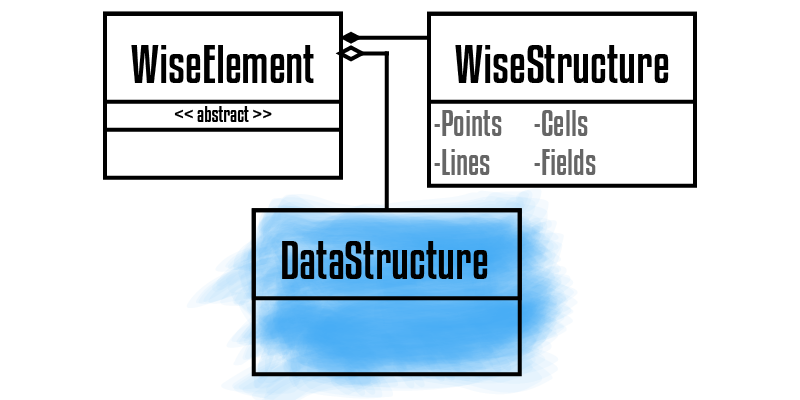
\includegraphics[width=1\textwidth]{images/Prancheta 2_2@4x.png}
			
		\end{itemize}
		
		\framebreak
		
		\begin{flushleft}
			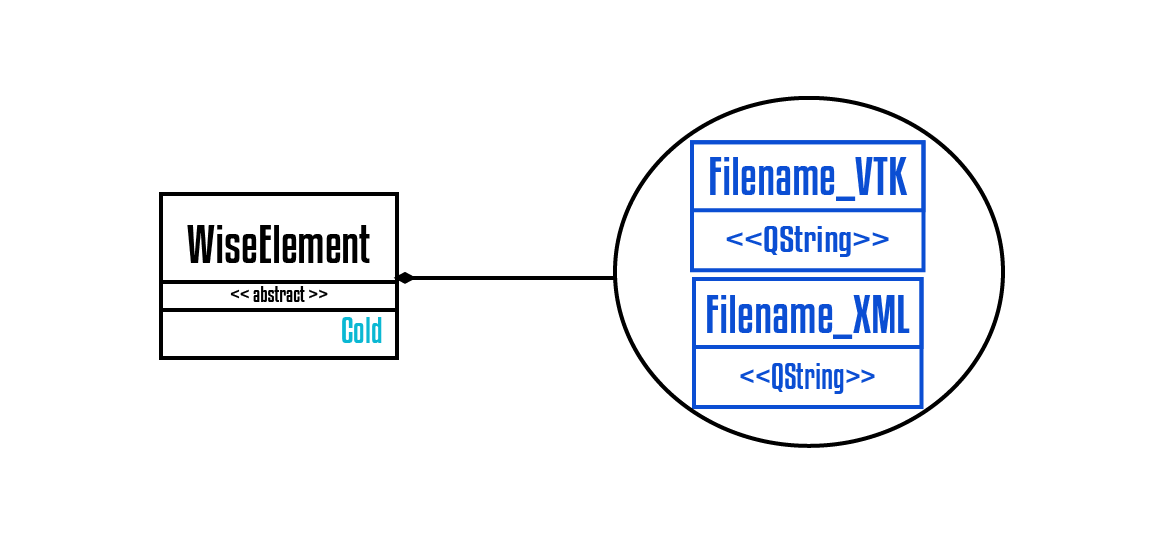
\includegraphics[width=0.4\textwidth]{images/Prancheta 8@4x.png}
		\end{flushleft}
		\begin{center}
			\item 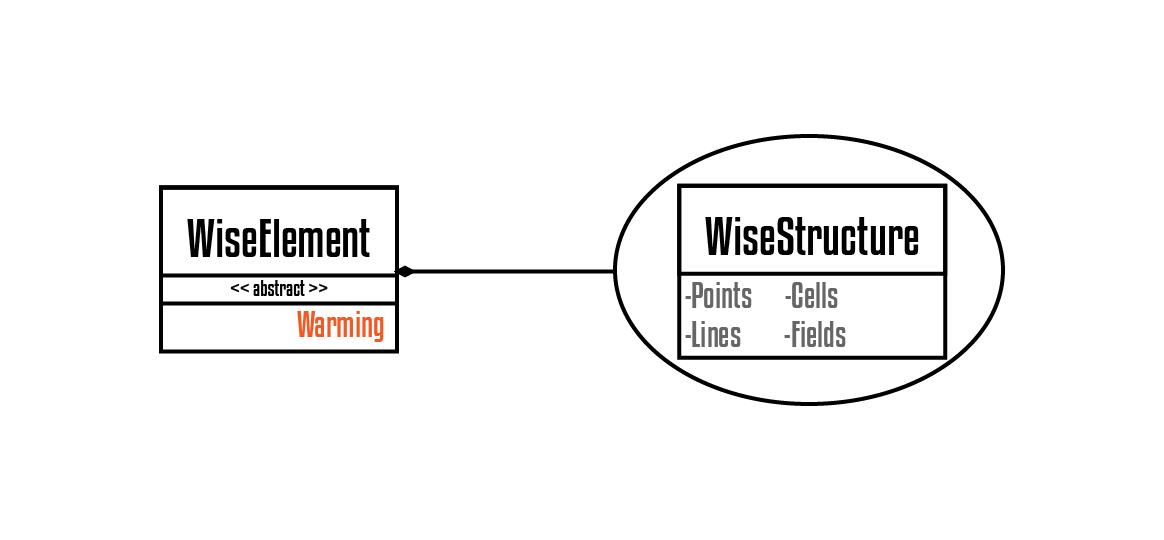
\includegraphics[width=0.4\textwidth]{images/Prancheta 9@4x.png}
		\end{center}
		\begin{flushright}
			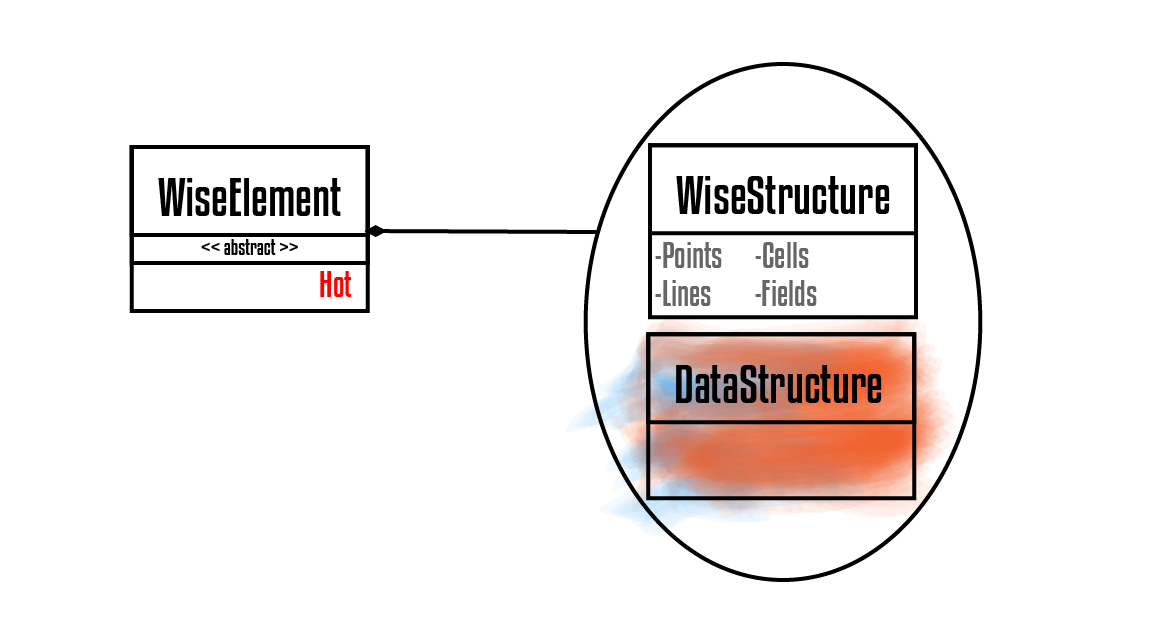
\includegraphics[width=0.4\textwidth]{images/Prancheta 10@4x.png}
		\end{flushright}
		
		\framebreak
		\begin{itemize}
			
			\item 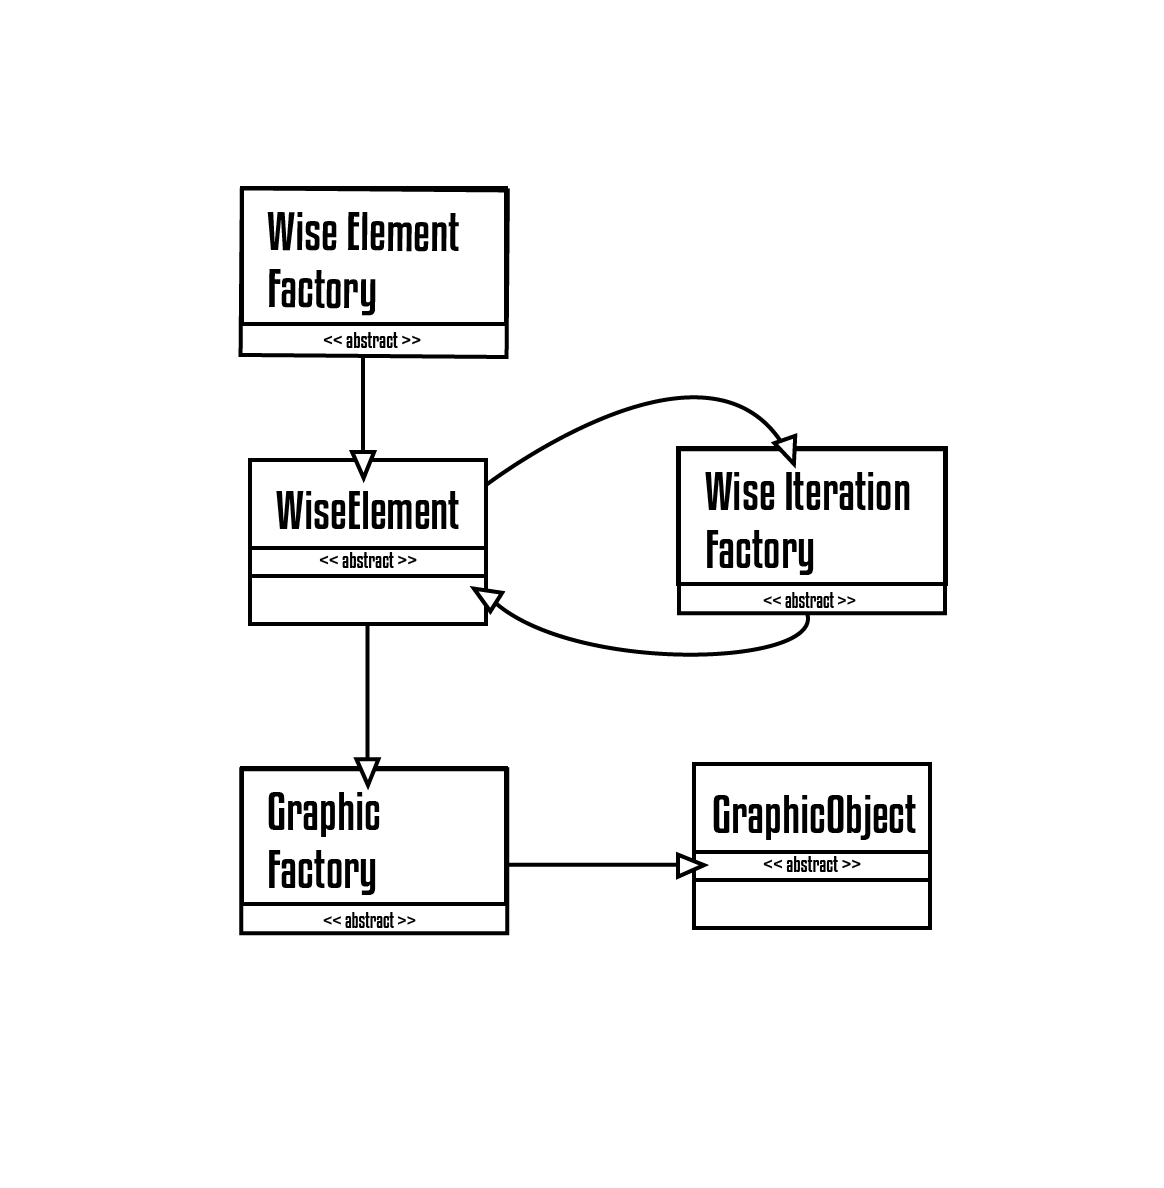
\includegraphics[width=0.6\textwidth]{images/Prancheta 11@4x.png}
			
		\end{itemize}
		
		\framebreak
		\begin{itemize}
			
			\item 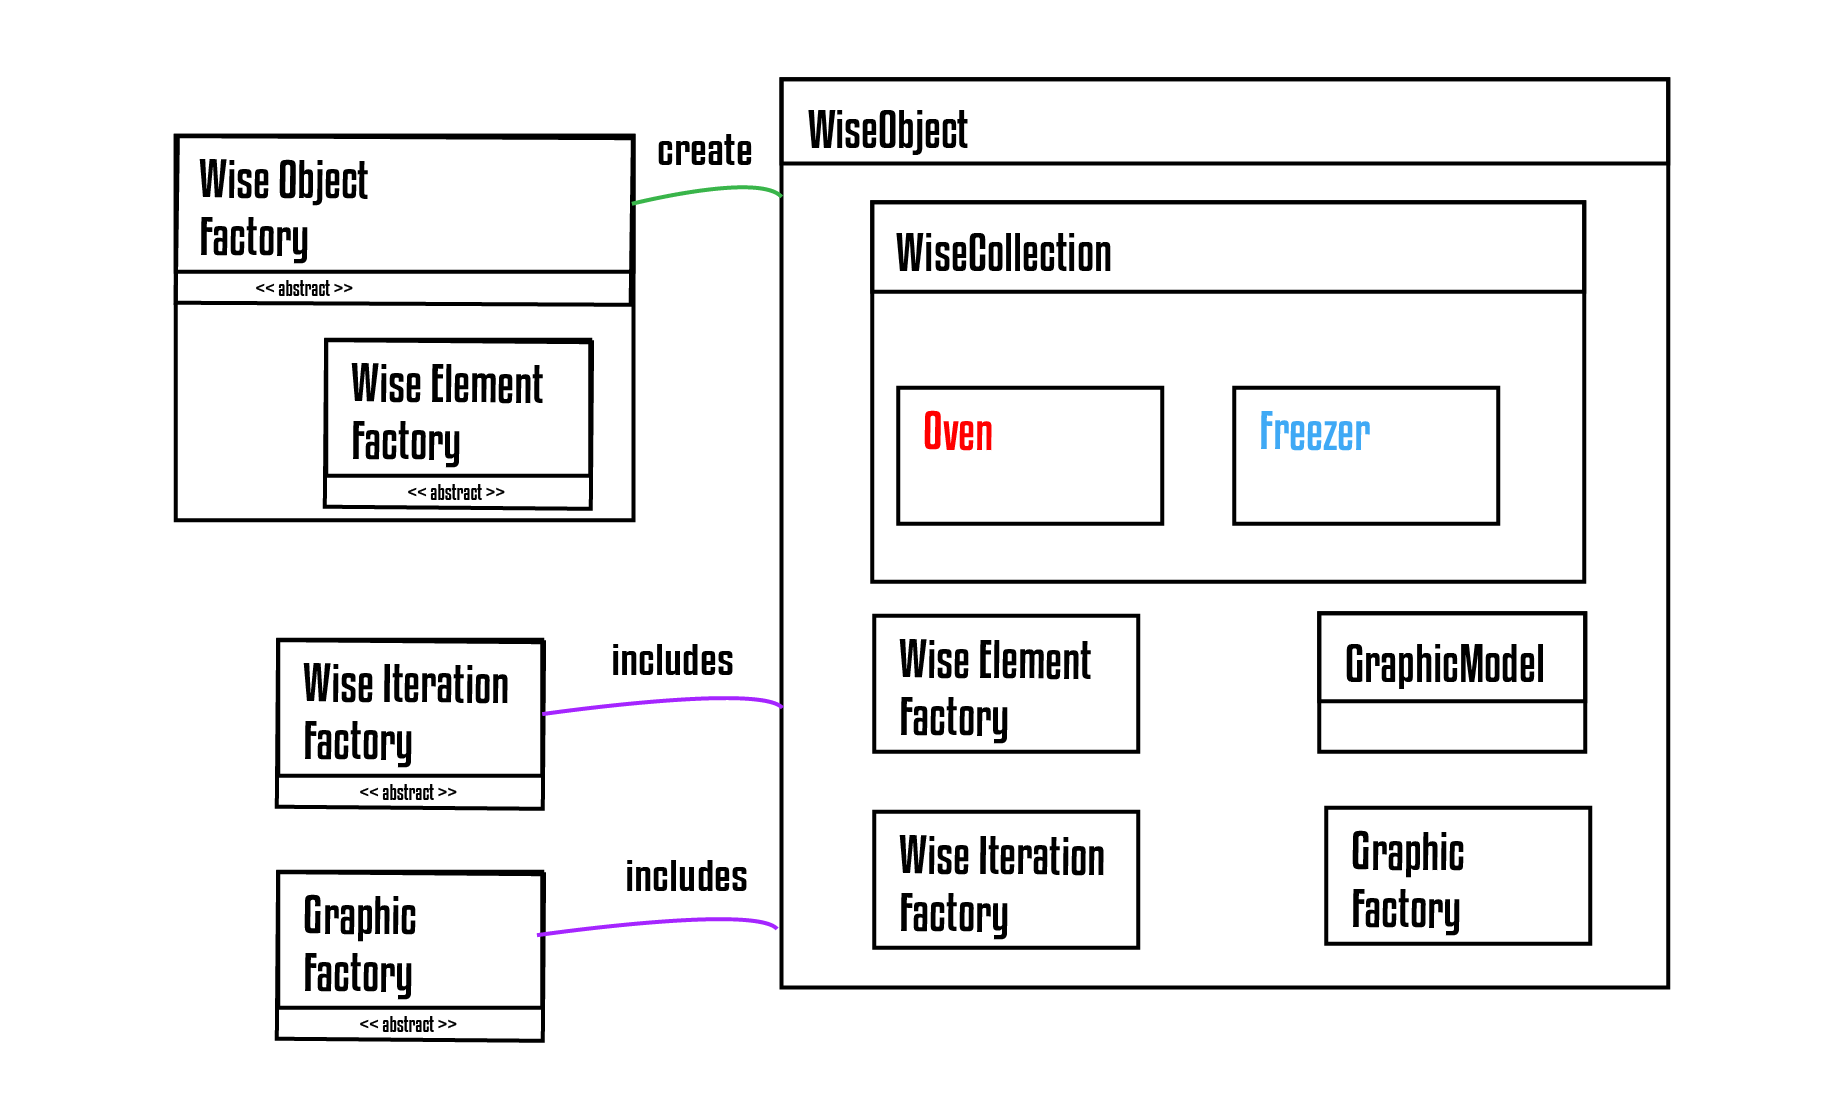
\includegraphics[width=0.6\textwidth]{images/Prancheta 13_1@4x.png}
			
		\end{itemize}
		
		\framebreak
		\begin{itemize}
			
			\item 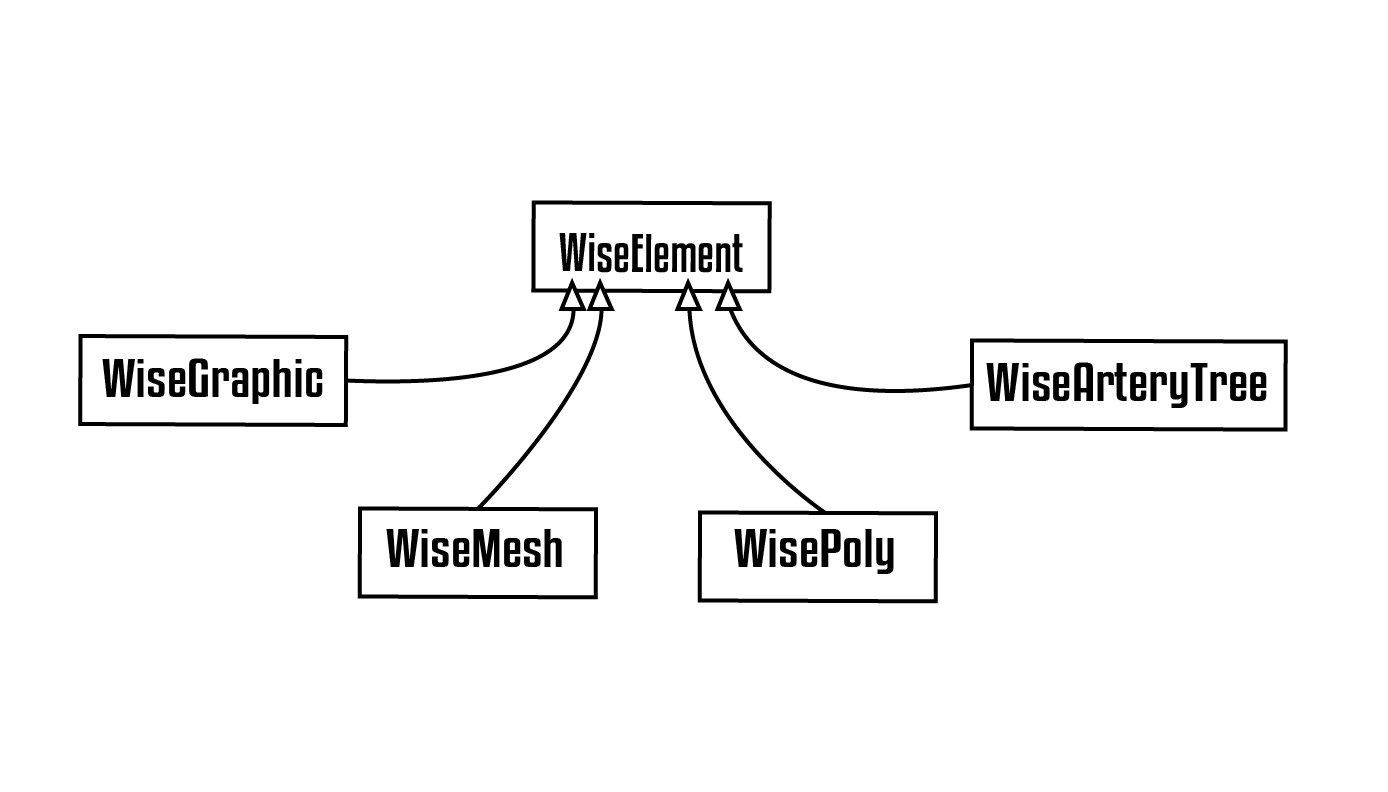
\includegraphics[width=0.6\textwidth]{images/Prancheta 13@4x.png}
			
		\end{itemize}
		
		\framebreak
		\begin{itemize}
			
			\item 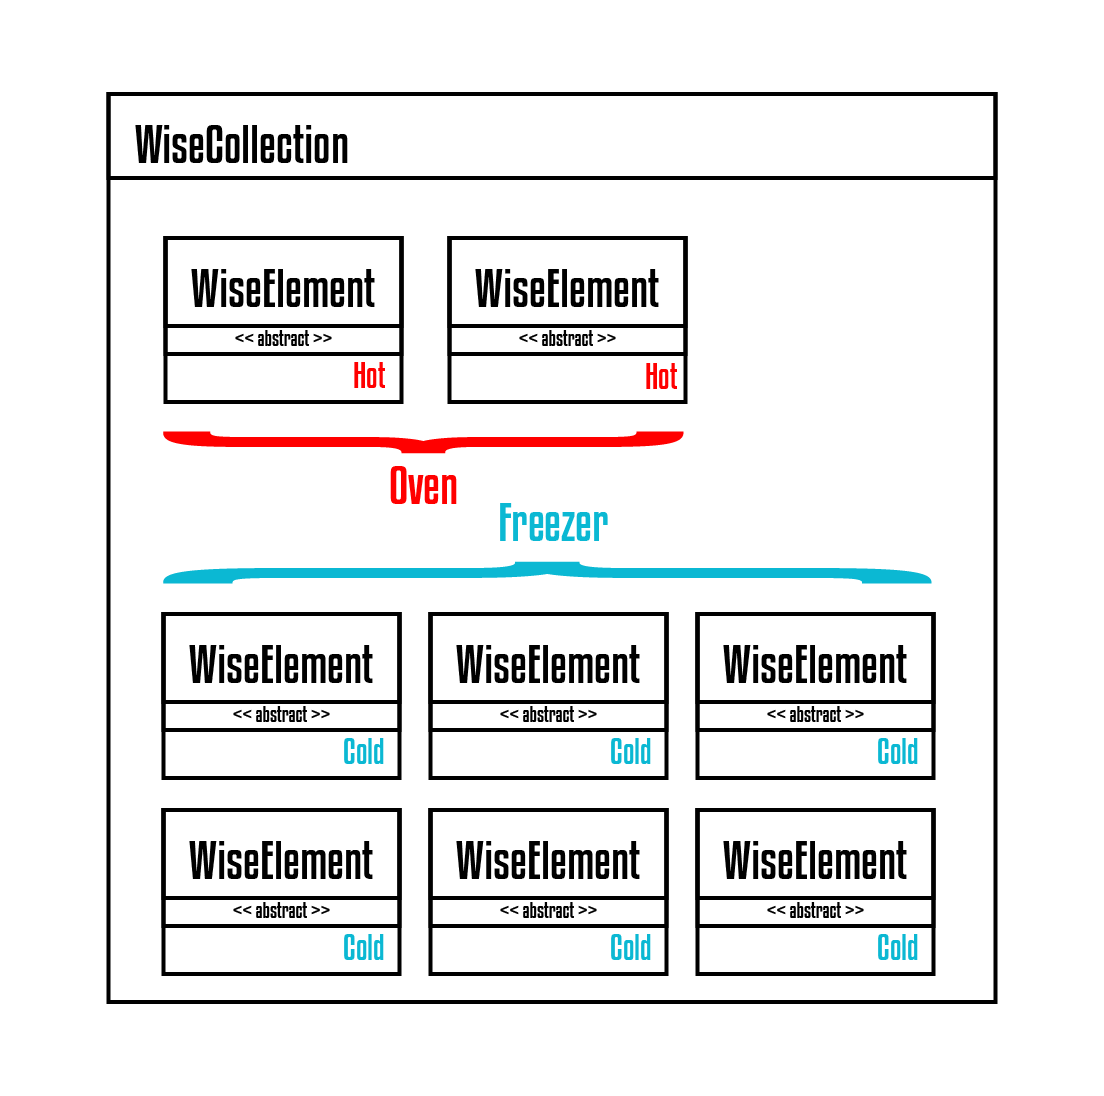
\includegraphics[width=0.6\textwidth]{images/Prancheta 17@4x.png}
			
		\end{itemize}
		
		\framebreak
		\begin{itemize}
			
			\item 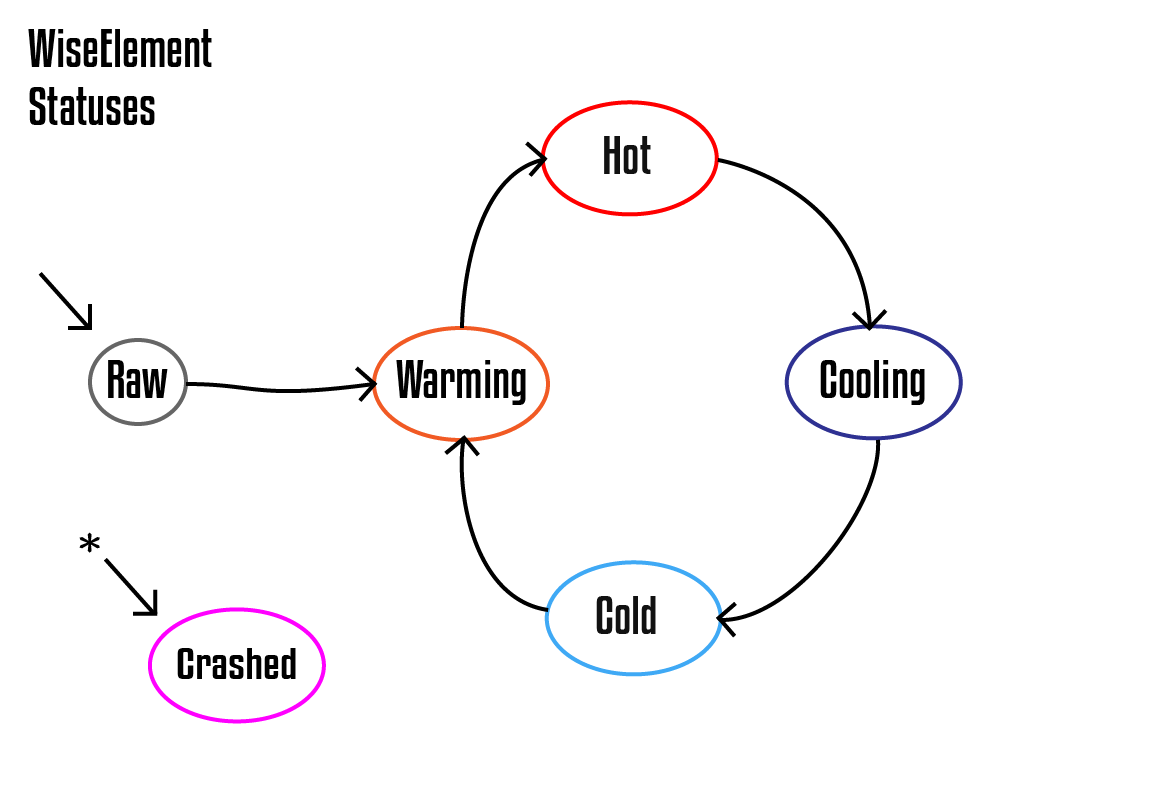
\includegraphics[width=0.6\textwidth]{images/Prancheta 7@4x.png}
			
		\end{itemize}
		
		\framebreak
		\begin{itemize}
			
			\item 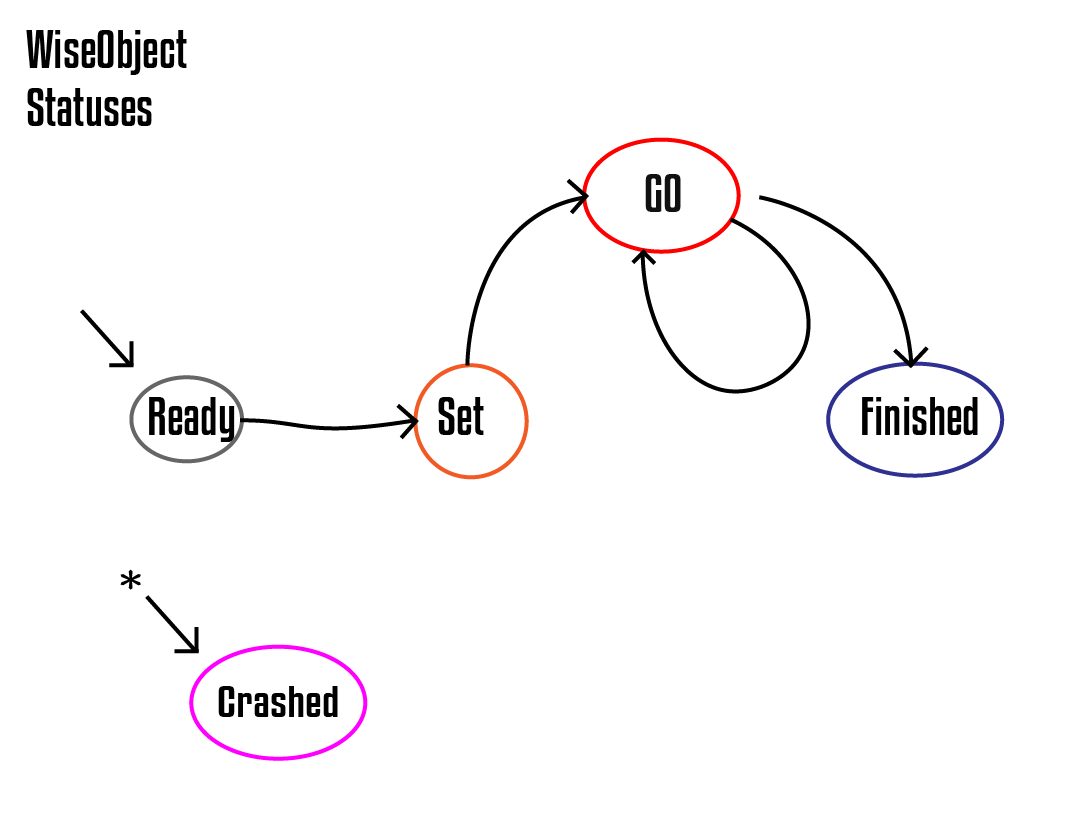
\includegraphics[width=0.6\textwidth]{images/Prancheta 16@4x.png}
			
		\end{itemize}
		
		\framebreak
		\begin{itemize}
			
			\item 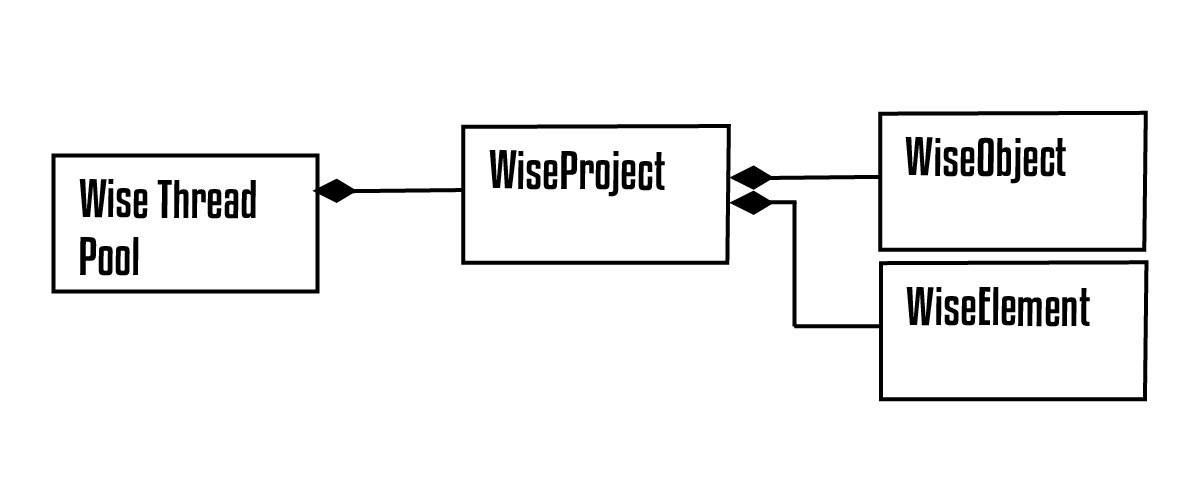
\includegraphics[width=0.6\textwidth]{images/Prancheta 14@4x.png}
			
		\end{itemize}
		
		\framebreak
		\begin{itemize}
			
			\item 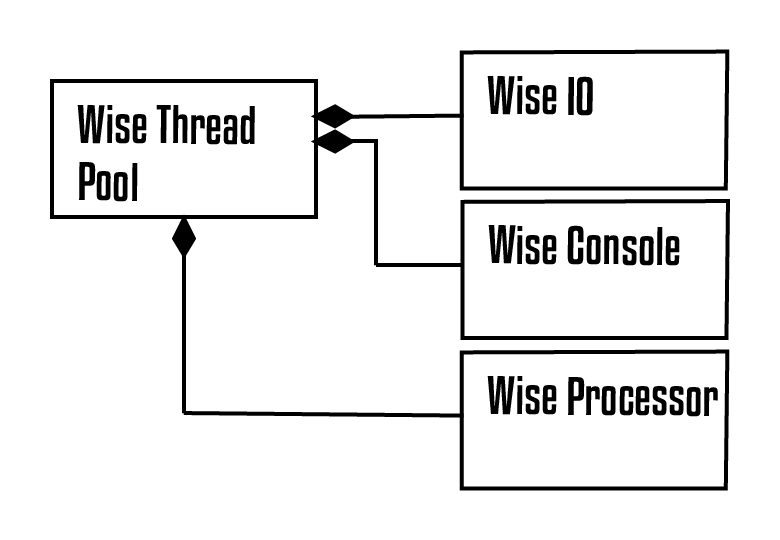
\includegraphics[width=0.6\textwidth]{images/Prancheta 15@4x.png}
			
		\end{itemize}
		
	\end{frame}
	
	\section{Resultados}
	\begin{frame}[allowframebreaks]
		\frametitle{Resultados}
		\begin{center}
			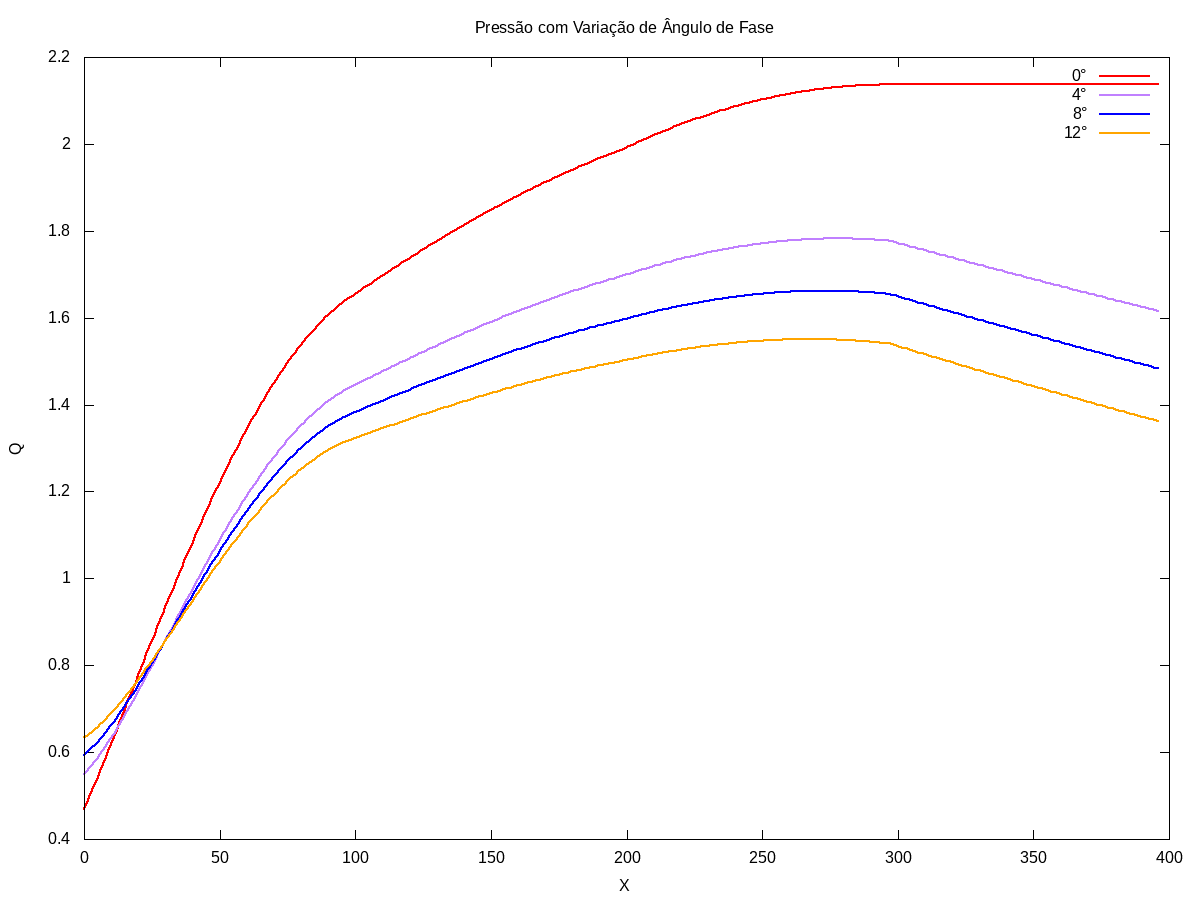
\includegraphics[width=0.4\textwidth]{images/48.png}
			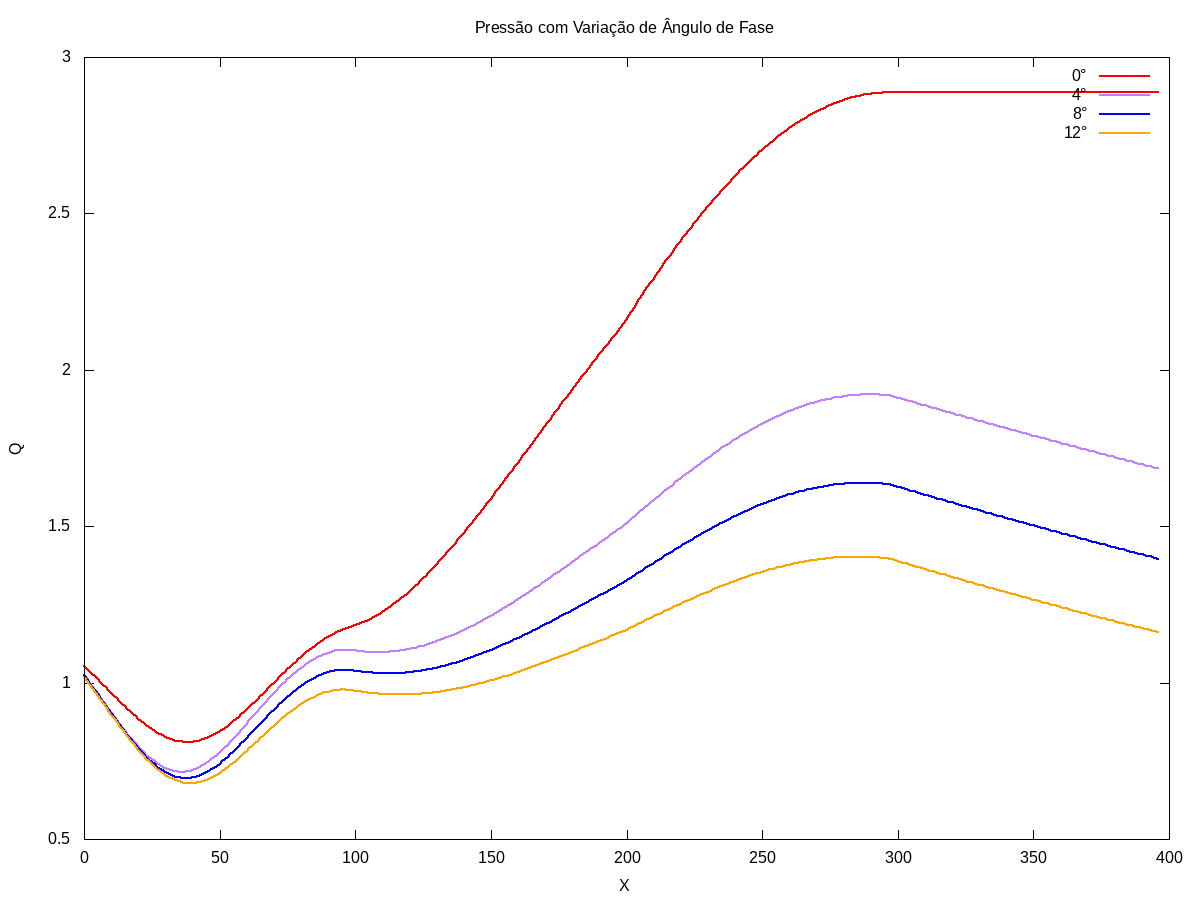
\includegraphics[width=0.4\textwidth]{images/49.png}
			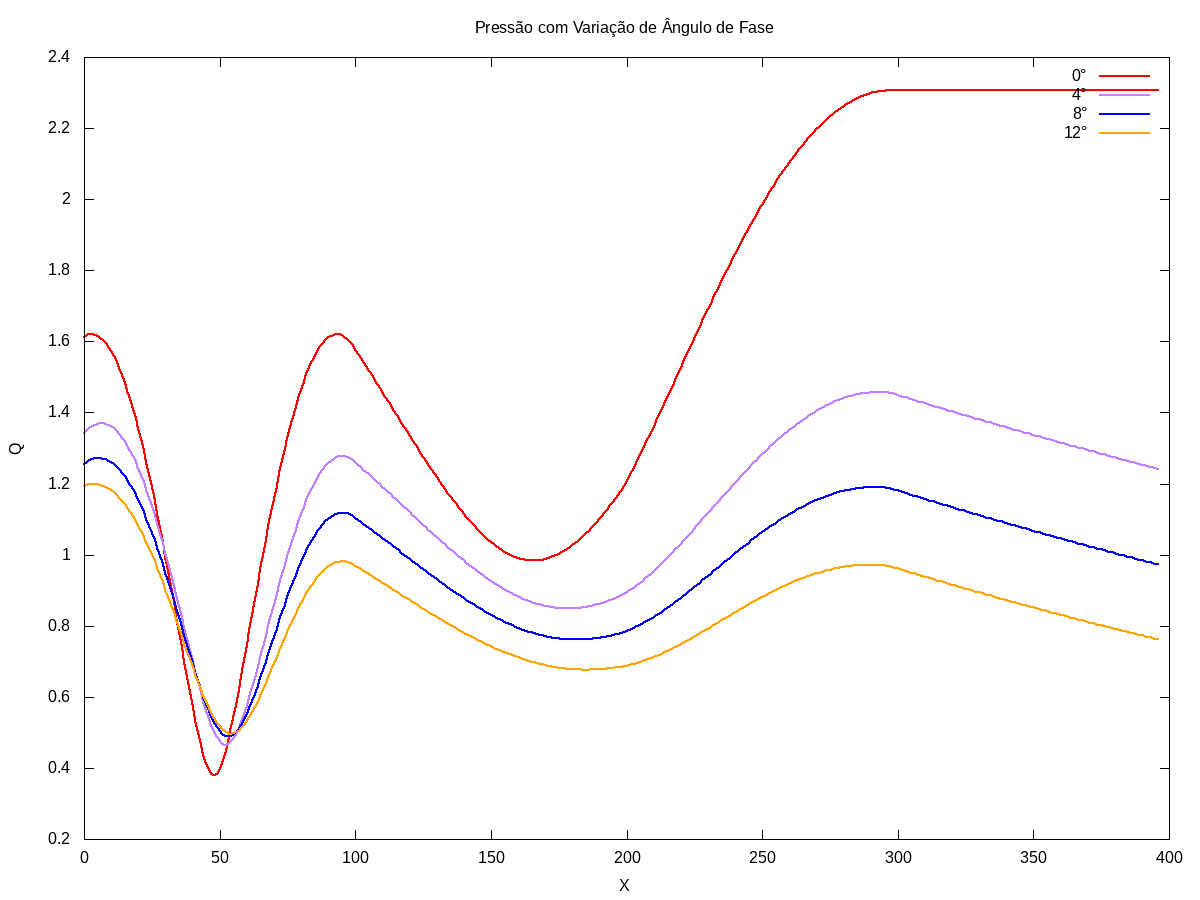
\includegraphics[width=0.4\textwidth]{images/50.png}
			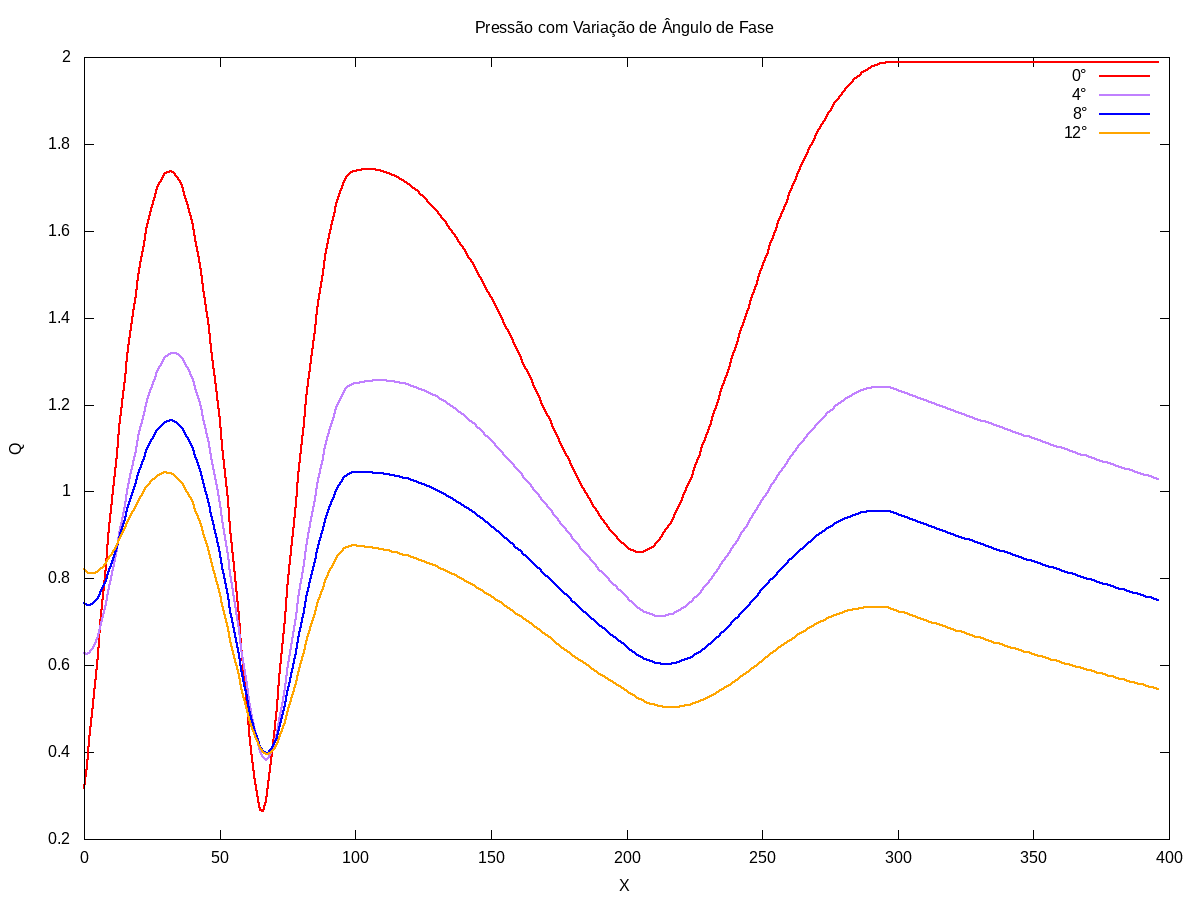
\includegraphics[width=0.4\textwidth]{images/51.png}
		\end{center}
		
		\framebreak
		
		\begin{center}
			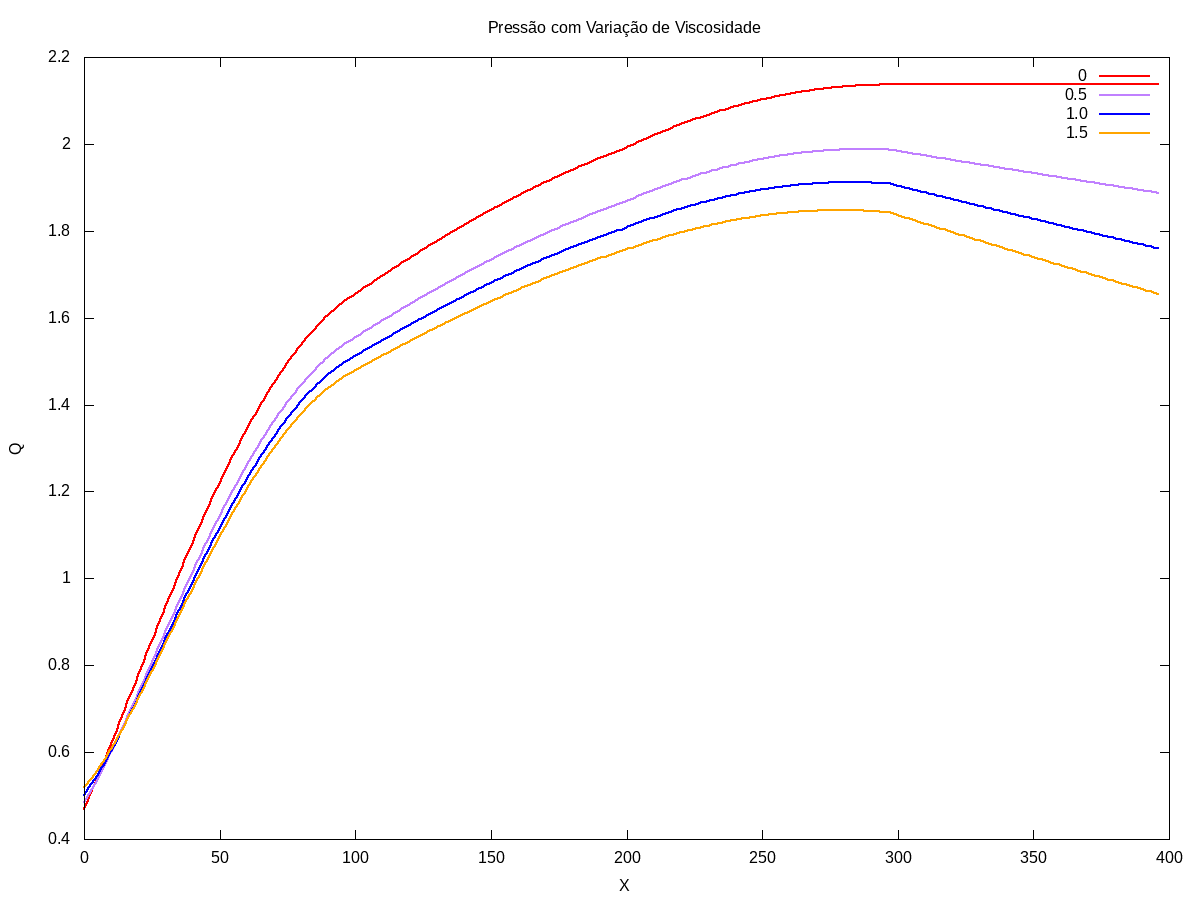
\includegraphics[width=0.4\textwidth]{images/52.png}
			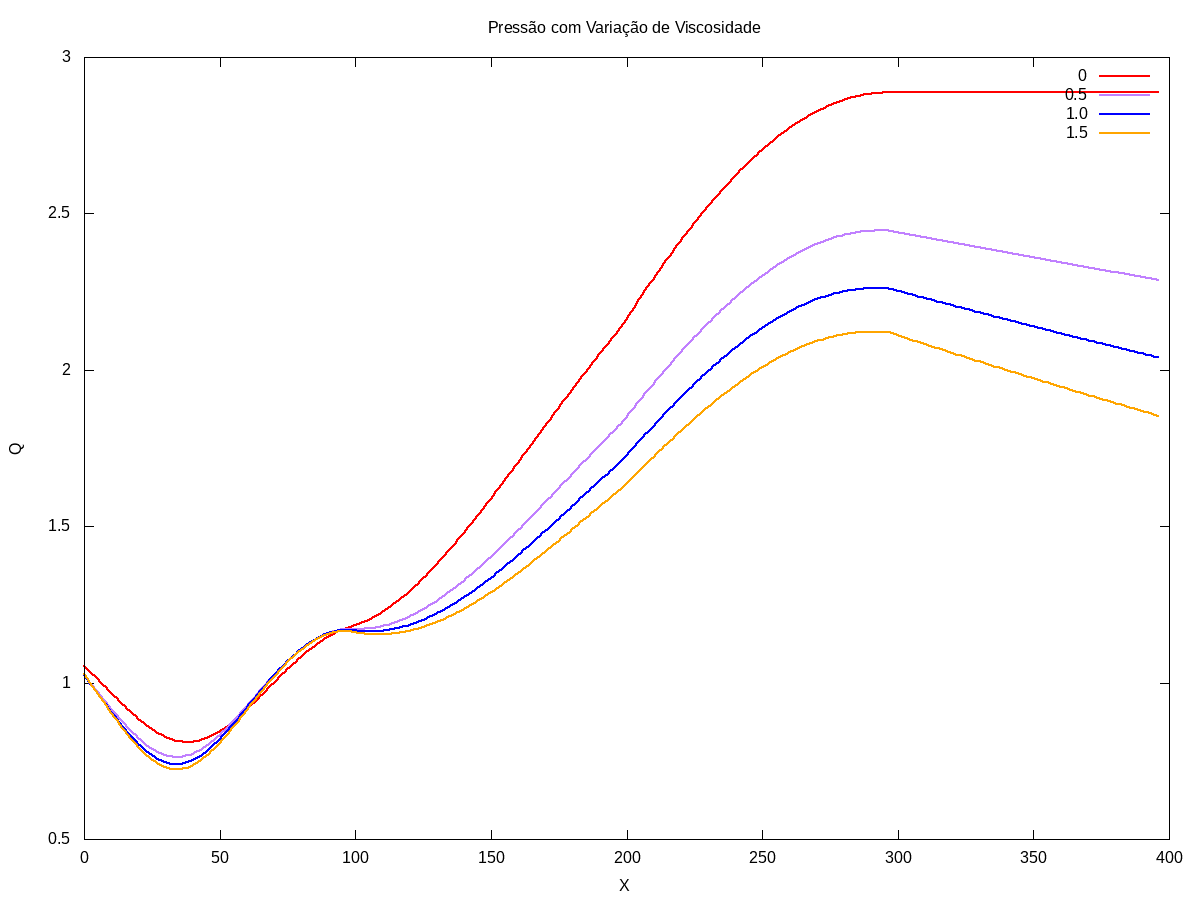
\includegraphics[width=0.4\textwidth]{images/53.png}
			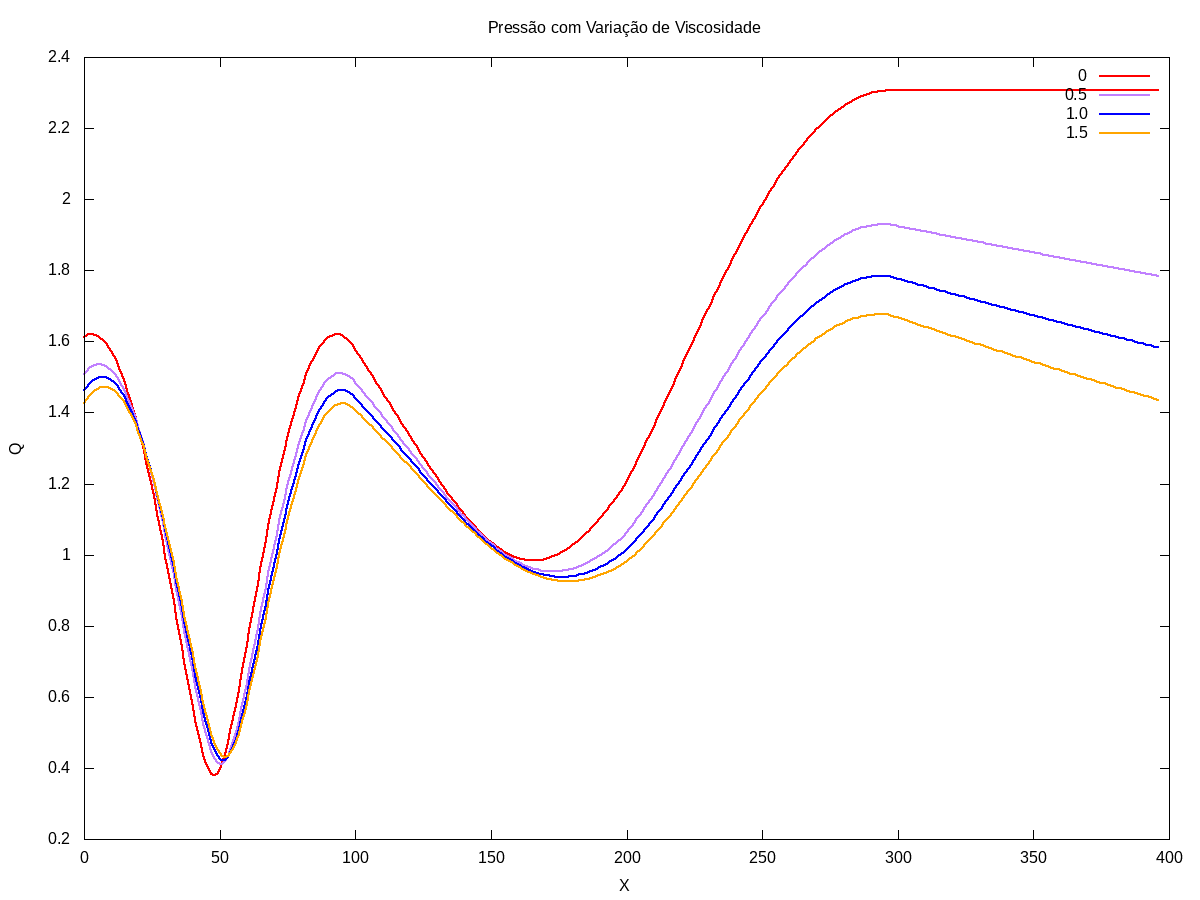
\includegraphics[width=0.4\textwidth]{images/54.png}
			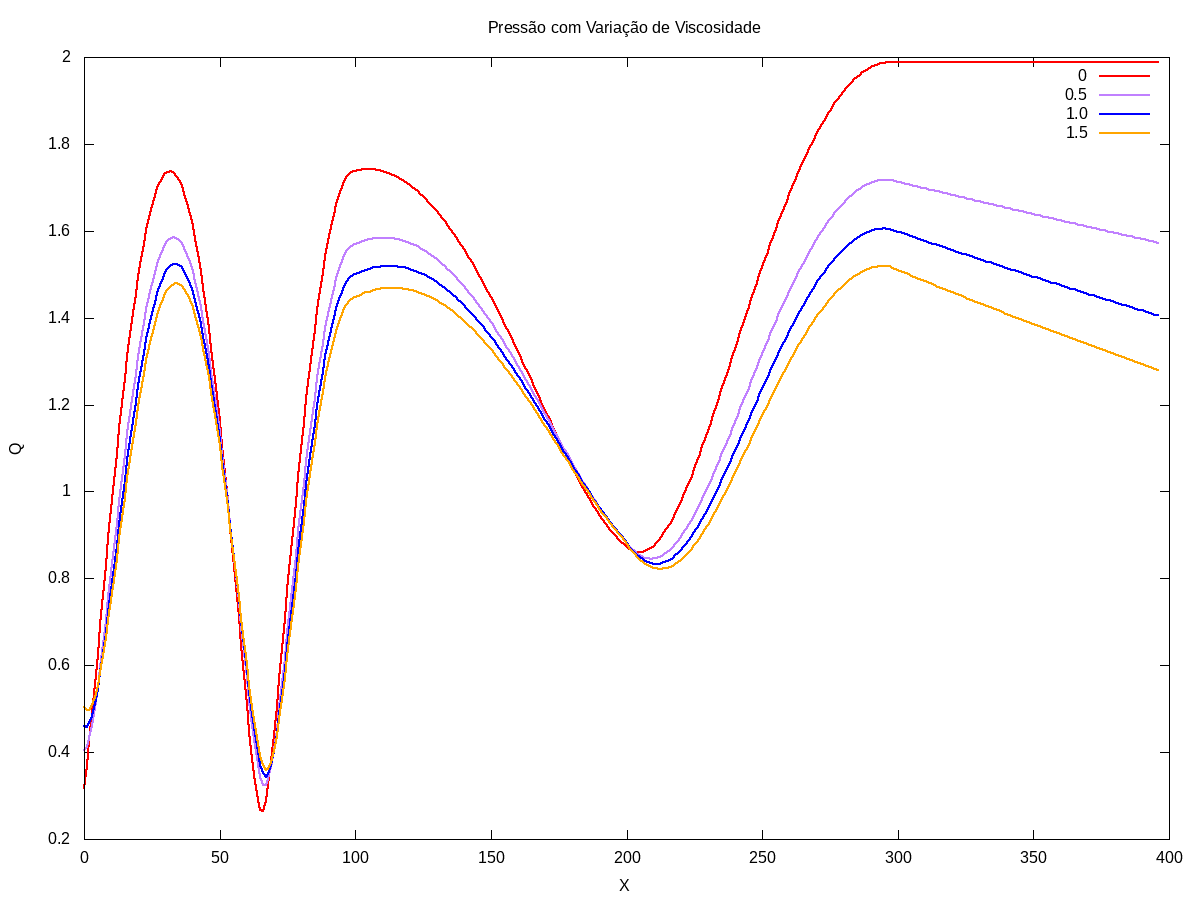
\includegraphics[width=0.4\textwidth]{images/55.png}
		\end{center}
	
		\framebreak
			
		\begin{center}
			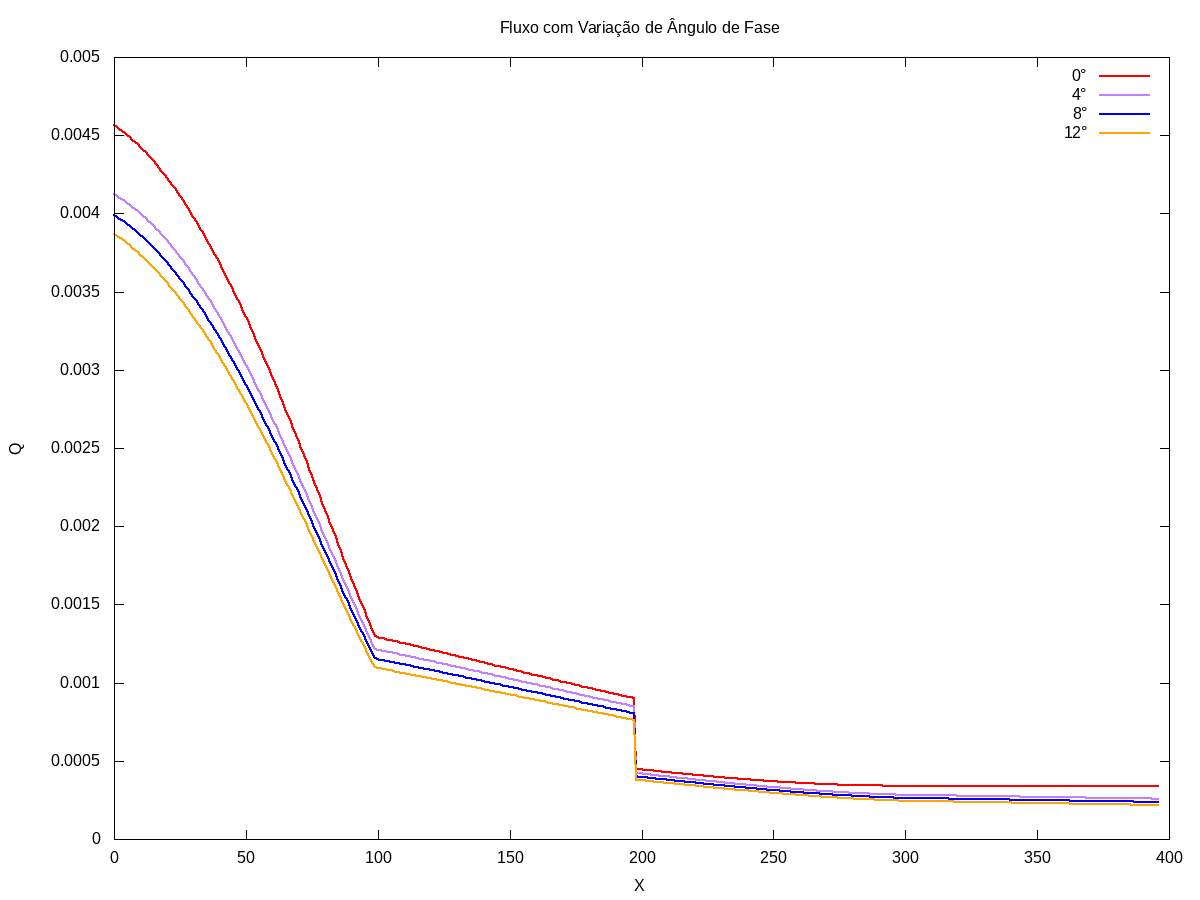
\includegraphics[width=0.4\textwidth]{images/56.png}
			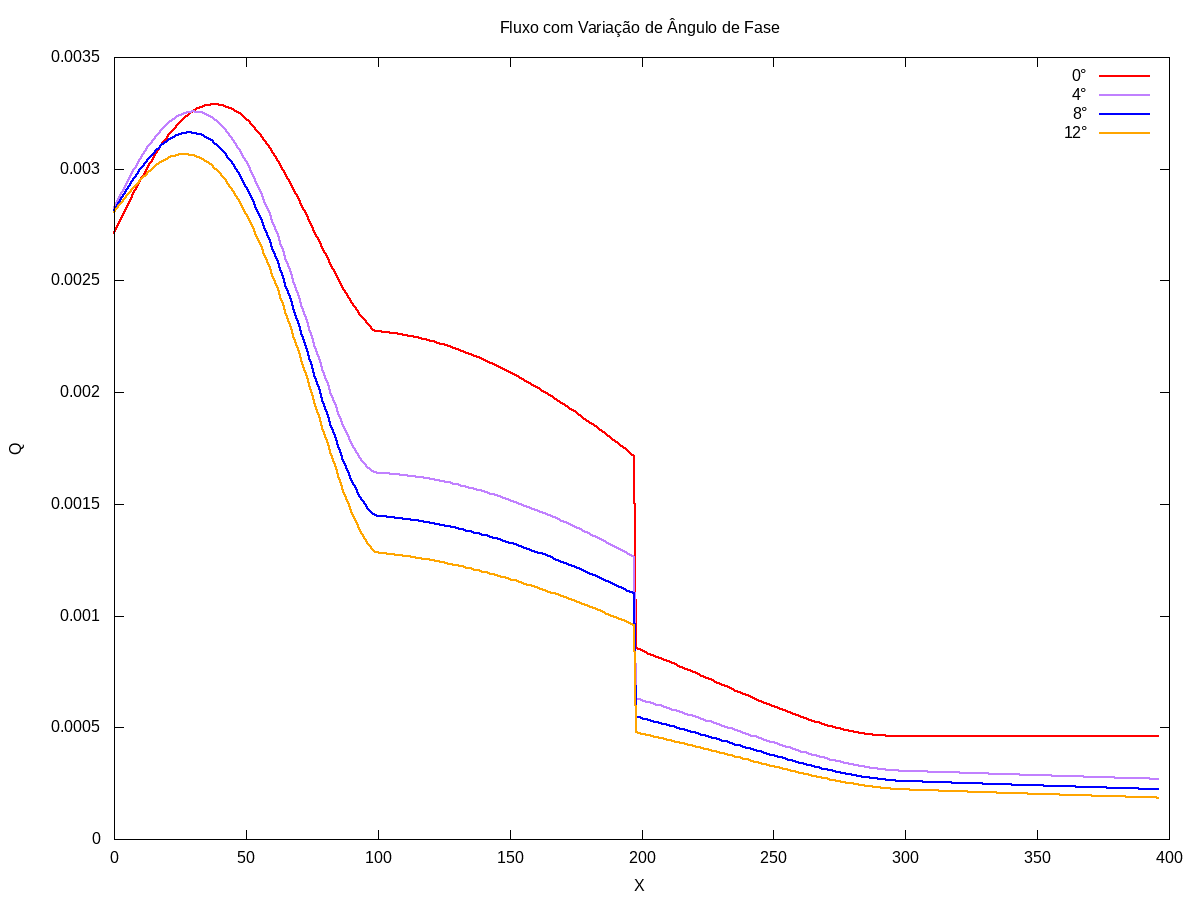
\includegraphics[width=0.4\textwidth]{images/57.png}
			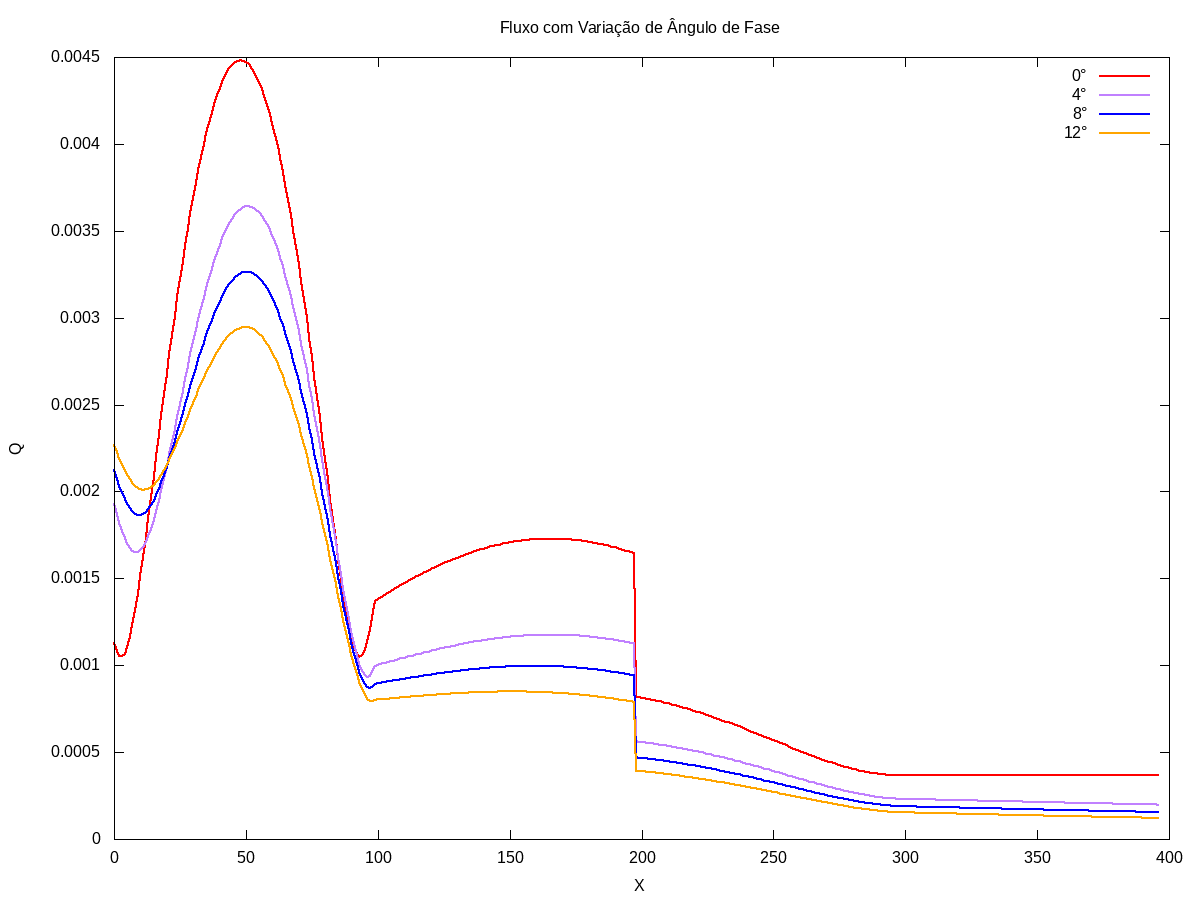
\includegraphics[width=0.4\textwidth]{images/58.png}
			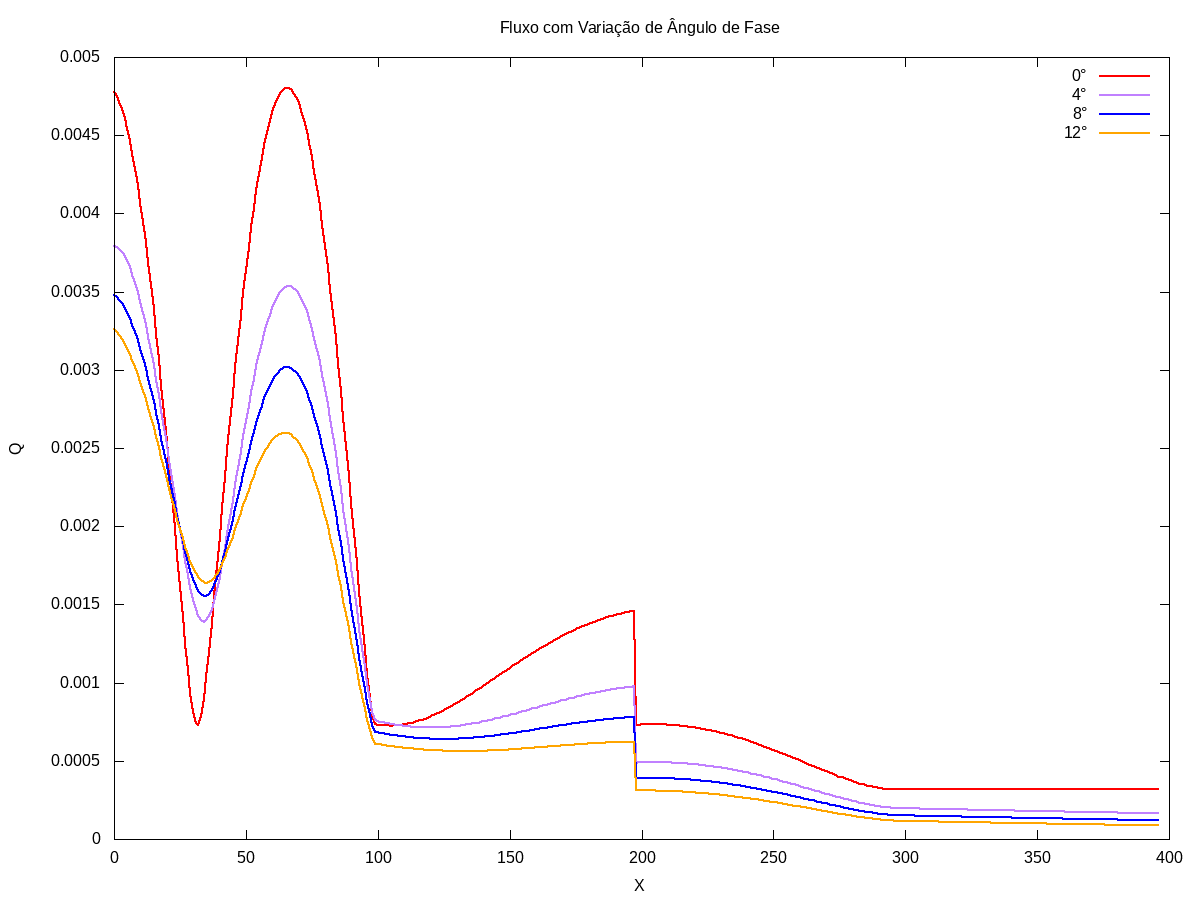
\includegraphics[width=0.4\textwidth]{images/59.png}
		\end{center}
		
		\framebreak
		
		\begin{center}
			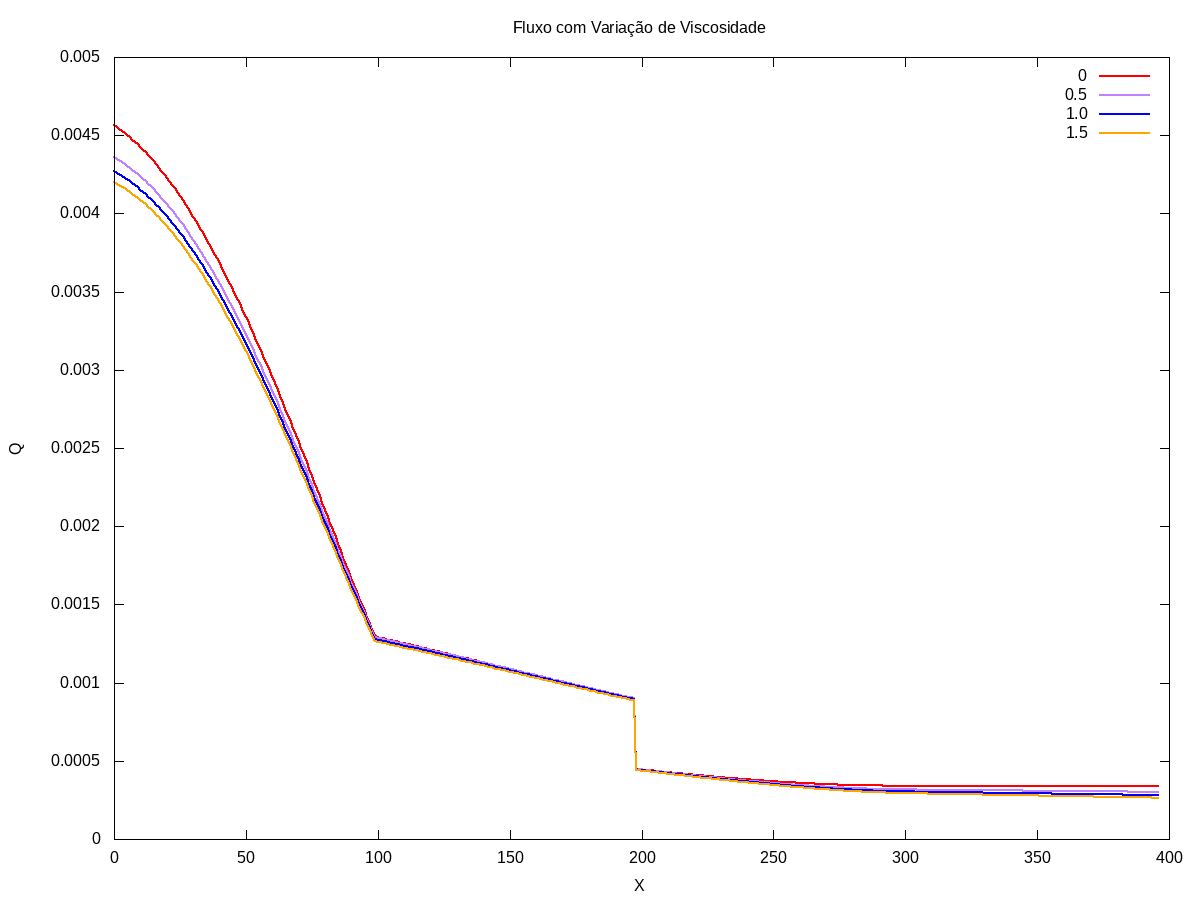
\includegraphics[width=0.4\textwidth]{images/60.png}
			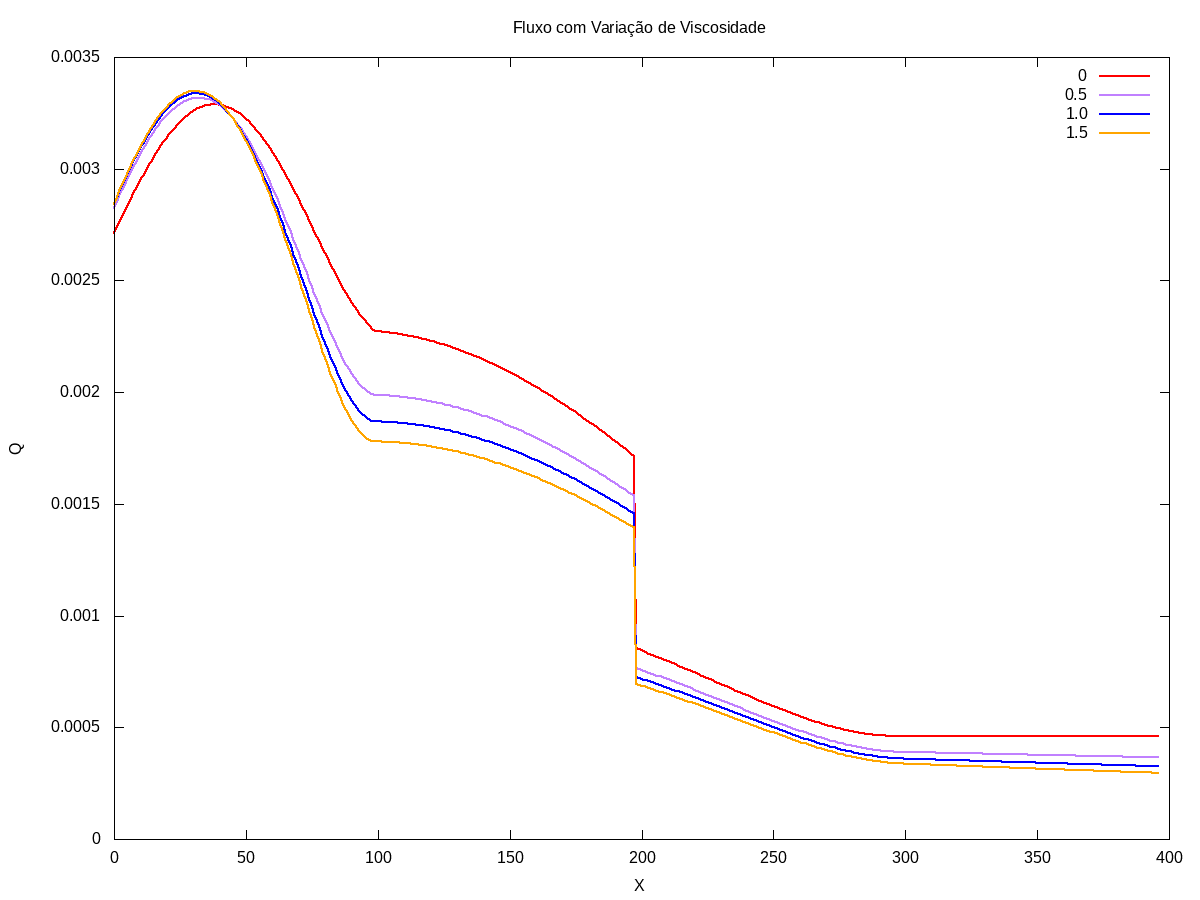
\includegraphics[width=0.4\textwidth]{images/61.png}
			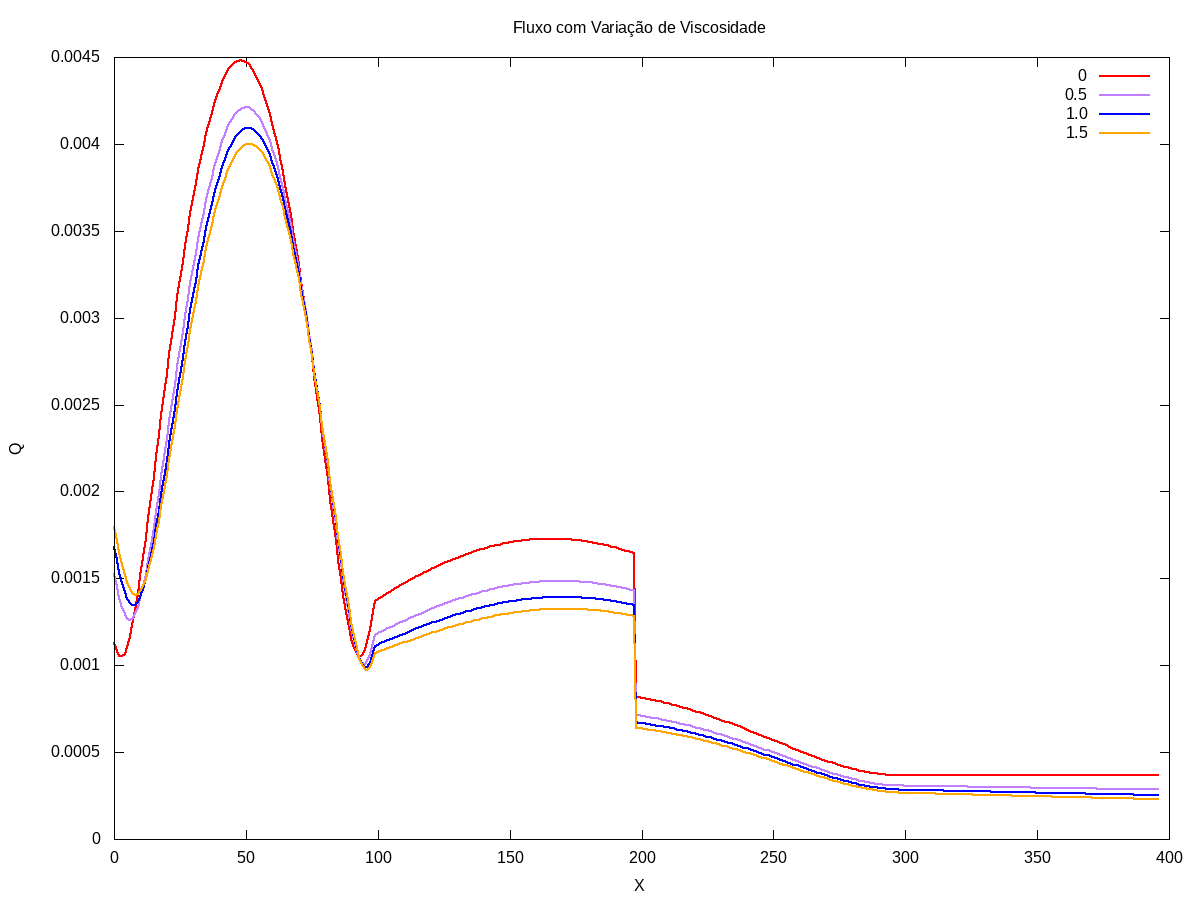
\includegraphics[width=0.4\textwidth]{images/62.png}
			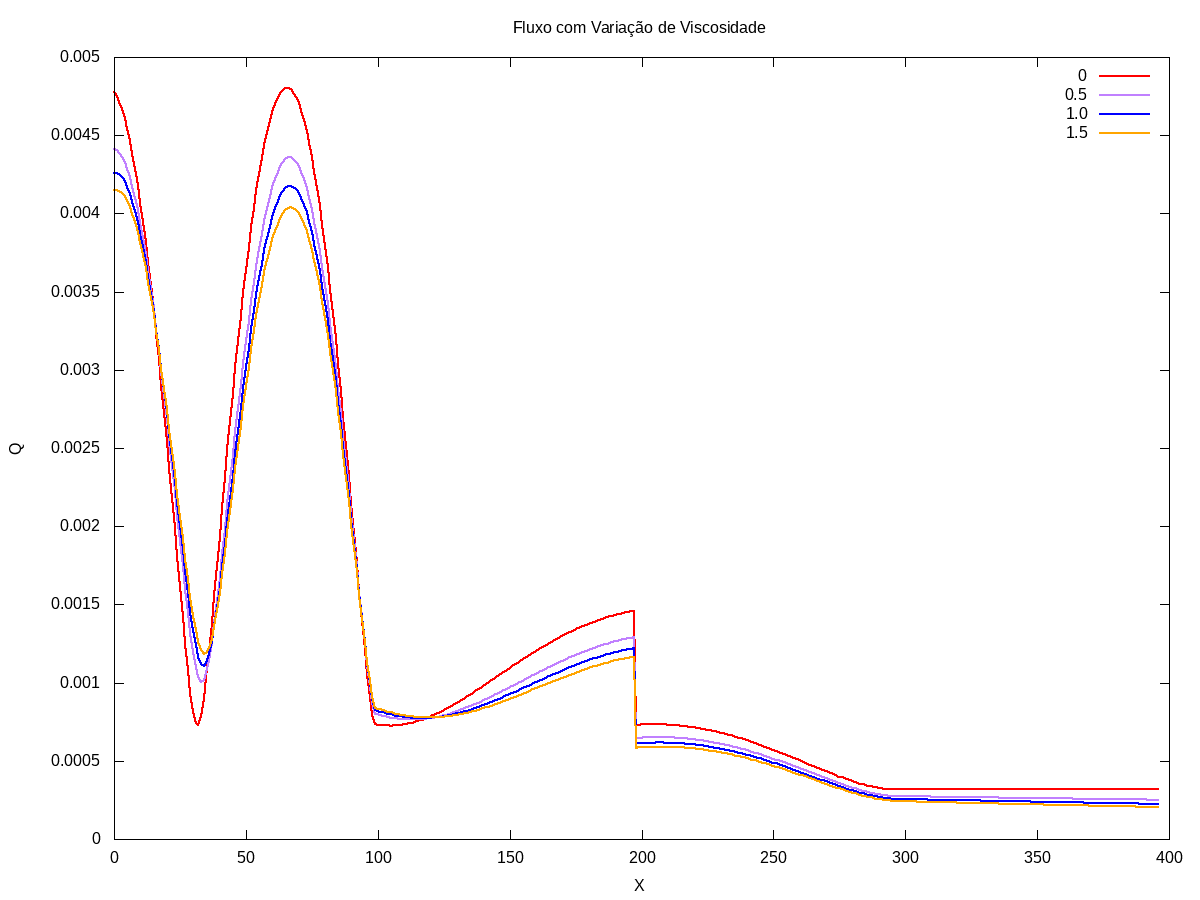
\includegraphics[width=0.4\textwidth]{images/63.png}
		\end{center}
	
	\end{frame}
	
	\section{Dissertação}
	\begin{frame}[allowframebreaks]
		\frametitle{Dissertação}
		
		\begin{itemize}
			\item Ferramenta Computacional
			\item Estrutura de dados
			\item  (Sinais e slots, paralelização)
			\item Lista de comandos
			\item Interface gráfica
			\item Resultados
			\item Fluxo
			\item Pressão
			\item Conclusão
		\end{itemize}
		
	\end{frame}
	
	\section{Cronograma}
	\begin{frame}[allowframebreaks]
		\frametitle{Cronograma}
		
		\begin{itemize}
			\item Mar: Ajustes dissertação + Fim da dissertação
			\item Abr: Ajustes finais
			\item Mai: Ajustes finais
		\end{itemize}
		
	\end{frame}
	
\end{document}